\documentclass[aspectratio=169]{beamer}
\usetheme{Madrid}

\title{How BRIDGES can help with Engagement}
\subtitle{}
\author{Kalpathi Subramanian$^1$, Erik Saule$^1$, Jamie Payton$^2$\\\texttt{krs@uncc.edu}, \texttt{esaule@uncc.edu}, \texttt{payton@temple.edu} }
\institute{$^1$The University of North Carolina at Charlotte\\$^2$Temple University}
\date{BRIDGES Workshop, May 30-June 1, 2023}

\setbeamertemplate{footline}

\usepackage{hyperref,graphicx}
\usepackage{subfloat}

\beamertemplatenavigationsymbolsempty % remove navigation symbols
\begin{document}


\begin{frame}
\titlepage
\end{frame}


\AtBeginSection[]
{
    \begin{frame}
        \frametitle{Table of Contents}
        \tableofcontents[currentsection]
    \end{frame}
}


\subsection{What makes a course engaging?}

\begin{frame}
	\frametitle{Engagement and Motivation}
\begin{itemize} 
	\item Well understood that student engagement is an important
		predictor of student achievement.
	\item Engagement can span many dimensions\footnote{Handelsman et al., 
	A Measure of College Student Course Engagment, Journal of Educ. Res., 2005}: 
		\begin{itemize}
			\item skills engagement
			\item participation/interaction engagement
			\item emotional engagement
			\item performance engagement
		\end{itemize}
	\item Engagement and motivation are closely tied to each other
	\item How do we motivate and engage students? 
	\item What engagement  strategies  can we use? 
%		Many models have been proposed, such as 
%		the MUSIC model of motivation  (Jones, 2009)
\end{itemize}
\end{frame}
\begin{frame}{Engagement Strategies}
\begin{itemize}
	\item \textbf{Active Learning:}
	\begin{itemize}
		\item Pair Programming
		\item Flipped classroom
		\item Group work/collaboration/Light Weight Teams
		\item Quizzes
	\end{itemize}
	\item \textbf{Content Based}
	\begin{itemize}
		\item Real world data integrated into  curriculum, demonstrate
			relevance
		\item Align with student interests, values, social relevance
	\end{itemize}
\vspace*{0.2in}
\textsl{\large BRIDGES focuses on \textbf{content based engagement}}
\end{itemize}
\end{frame}
\begin{frame}{The MUSIC Model of Engagement}
\footnote{ Jones, B.D, Motivating Students to Engage in Learning: The MUSIC Model of Academic Motivation, Intl. Journal of Teaching and Learning in Higher Ed., 2009}
\centering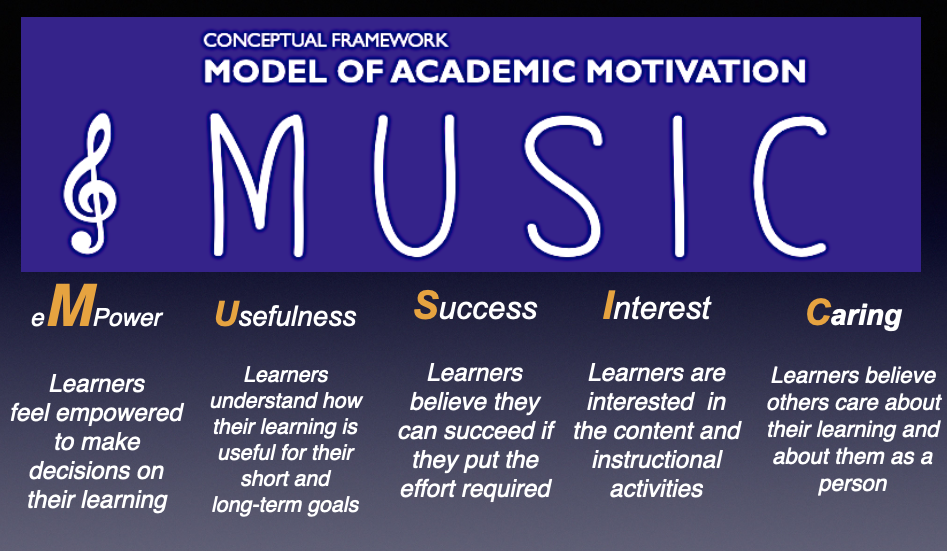
\includegraphics[width=4in]{figs/music_model.png}
\end{frame}
\begin{frame}{Engaging Students: Experiences from an OOP Course
\footnote{Subramanian et al., Influence of Course Design on Student Engagement and Motivation in an Online Course, ACM SIGCSE 2020}}
\begin{block}{Two semesters of a project based OOP course, using
student  reflections after each course module}
\end{block}
\begin{itemize} 
	\item e\textbf{M}powerment: Project choice, freedom to be creative, 
		experimentation and tinkering
	\item \textbf{U}sefulness: Working with real-world data/tools, team
		environment
	\item \textbf{S}uccess: Assignments with clear instructions, predictability,
		reflect on personal successes/failures, feedback, challenges (in a good way!)
	\item \textbf{I}nterest: Fun factor,  games, real world images used
		as part of course
	\item \textbf{C}aring: Sensitive to student needs, prompt feedback, deadline
		flexibility
\end{itemize}
\end{frame}
\begin{frame}{Engagement Using BRIDGES: Visual and Interactive}
\begin{itemize}
	\item BRIDGES generates \textbf{visualizations} of data structures 
	(\textbf{that students implement!}), algorithm outputs
		as a mechanism for engaging students.
	\item Visualizations of classic CS concepts can be helpful in making
		them real and more meaningful. 
	\item Student feedback has been very positive, appreciating the features
		of BRIDGES that enables them to \textbf{see what they code and produce}.
\end{itemize}
  \begin{columns}
    \begin{column}{.47\linewidth}
      \begin{block}{\href{http://bridges-cs.herokuapp.com/assignments/137/kalpathi60}{\underline{Indexing USGS Earthquake}}}
        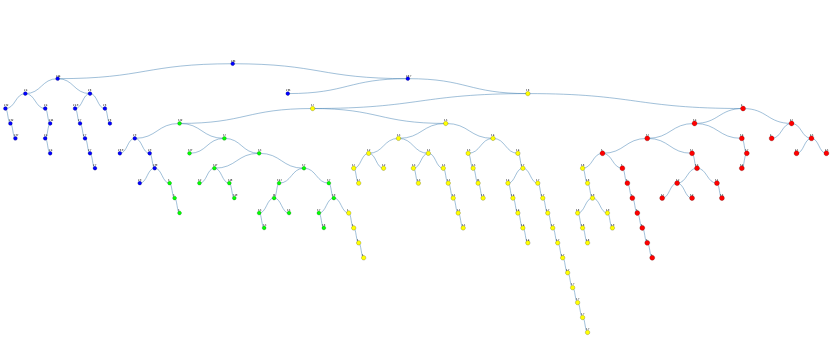
\includegraphics[width=\linewidth]{figs/BSTEq.png}
      \end{block}
    \end{column}
    \begin{column}{.47\linewidth}
      \begin{block}{\href{http://bridges-cs.herokuapp.com/assignments/1002/bridges_public}{\underline{Bacon Number [IMDB Data]}}}
        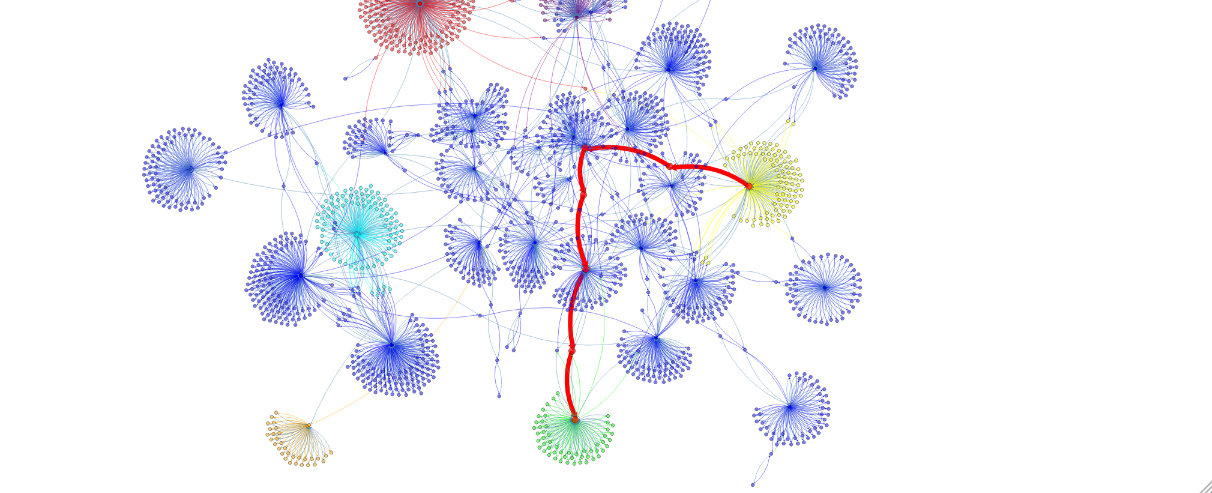
\includegraphics[width=\linewidth]{figs/BaconNumber.png}
      \end{block}
    \end{column}
  \end{columns}  
\end{frame}
%\begin{frame}
%  \frametitle{Activity: Discussion}

%\begin{block}{What are your thoughts on engaging students as part of course activities?}
%\end{block}
%\begin{itemize}
%\item  How do you engage your students? 
%\item  What tools/techniques have you used in the past to motivate s
%		tudents?
%\item Is there something you havent tried and would like to try?
%\end{itemize}
%\end{frame}

%\subsection{Making it interactive/visual}

%\begin{frame}{Making it Interactive/Visual}
%\begin{itemize}
%       Data on this is somewhat mixed on algovis, but
%		for some 
%		problems/applications that  has spatial and/or temporal content,
%		it makes sense to view the results.
%	\item Interactive applications is a more attractive approach to 
%		experimentation - changing parameters to see its effect on a 
%		phenomenon, solution, performance.
%  Game based applications are appreciated, but its important to tie that
%  to objectives, eg., board based games lets you practice conditionals,
%  iterations, 2D arrays
%\end{itemize}
%\end{frame}
%\begin{frame}{Activity}
%\begin{itemize}
%	\item Review BRIDGES tutorials 
%\end{itemize}
%\end{frame}
%
%\subsection{Making it real!}
\begin{frame}{Engagement Using BRIDGES: Use Real-World Data}

%\begin{frame}{Make it Real!}
\begin{itemize}
\item Using \textbf{real-world data} in course work is an important engagement tool
\item Students respond to working with data from real-world scenarios/data:
	weather/climate, maps, medical, census, books, music, videos, games
\item Data is everywhere, the \textbf{harder part is} 
	\begin{itemize}
		\item Accessing data in a ready-to-use form for course work
		\item Mapping the right data to course work to meet objectives.
	\end{itemize}
\item BRIDGES supports a number of datasets ready to use in early CS courses:
	\begin{itemize}
	\item \textbf{Earthquake Data:} \\
		\textsl{List$<$EarthquakeUSGS$>$eq\_list = bridges.getDataSource().getEarthquakeUSGSData(100) }
	\item \textbf{IMDB Actor-Movie Data:}\\
		\textsl{List$<$ActorMovieIMDB$>$am\_list} \textsl{= bridges.getDataSource().getActorMovieIMDBData(1813) }
	\item \textbf{Open-Street Map Data:}\\
		\textsl{OsmData osm\_data = bridges.getDataSource().getOsmData("Charlotte, North Carolina", "default")}

	\end{itemize}
\end{itemize}
\end{frame}
\begin{frame}{Results: Students in BRIDGES sections gained more knowledge}
  \begin{columns}
    \column{.49\linewidth}
    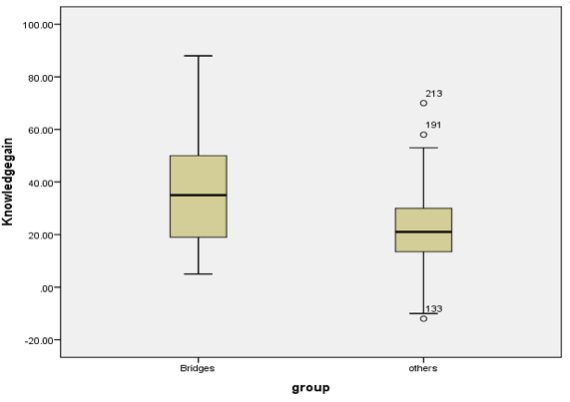
\includegraphics[width=\linewidth]{fig/knowl_gain_f14.png}

    \center Fall 2014

    \column{.49\linewidth}
    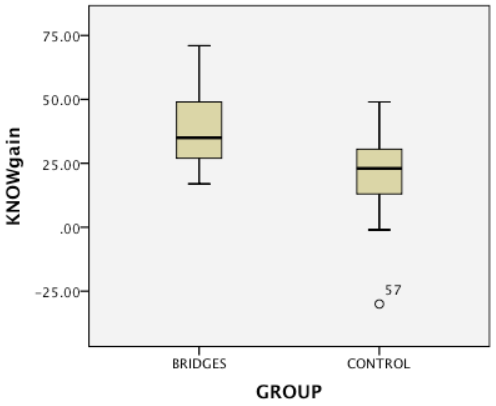
\includegraphics[width=\linewidth]{fig/knowl_gain_s15.png}

    \center Spring 2015
  \end{columns}
  \end{frame}

\begin{frame}{Results: Students in BRIDGES sections progressed faster in CS}
  \begin{figure}[htp]
    \centering
    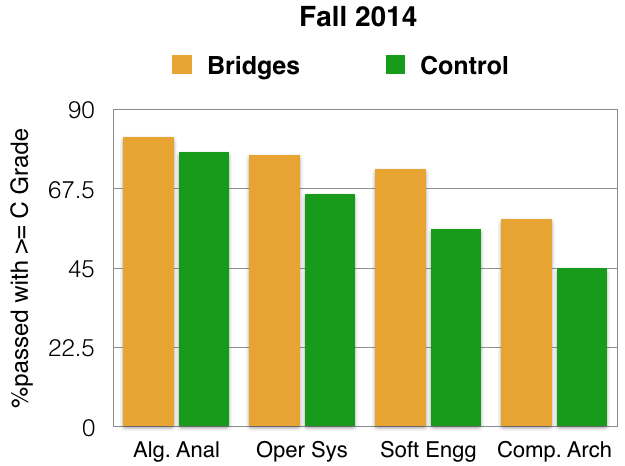
\includegraphics[width=.32\linewidth]{fig/prog_f14.png}
    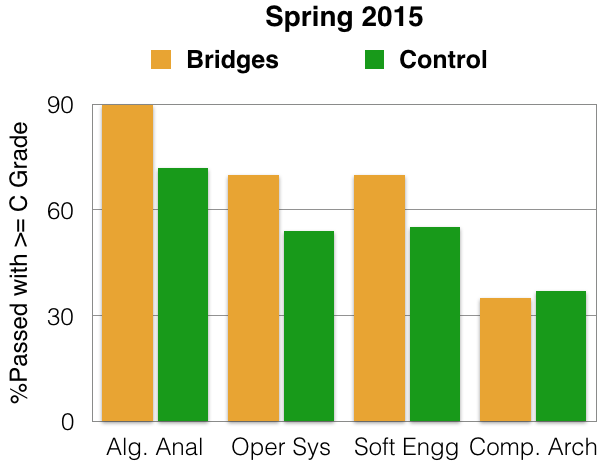
\includegraphics[width=.32\linewidth]{fig/prog_s15.png}
    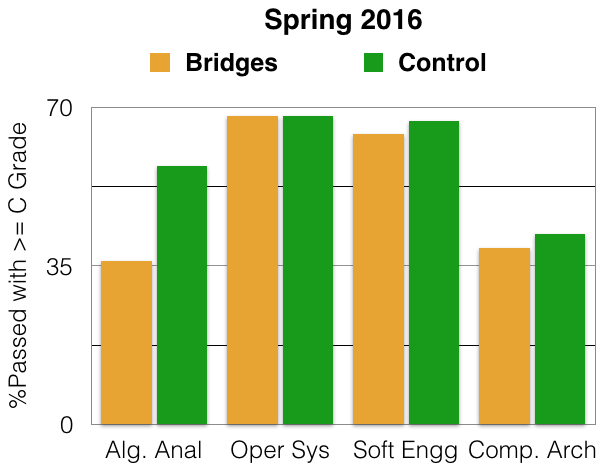
\includegraphics[width=.32\linewidth]{fig/prog_s16.png}
    \caption{Comparing long-term student achievement between students who used the
      BRIDGES toolkit in the Data Structures course vs. Control group. The evaluation was
      performed with 3 cohorts of students (Fall 14, Spring 15, Spring 16).

    Analysis performed Spring 2019.
    }
    \label{fig:long_study}
  \end{figure}
\end{frame}

\end{document}
%\framebox{
%\centering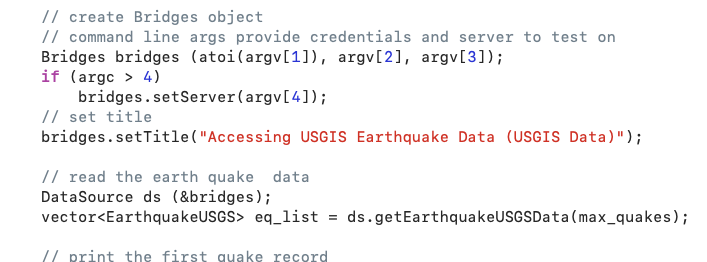
\includegraphics[width=3.5in]{figs/eq_snippet.png}
%}
\subsection{The power of choice}
\begin{frame}{The Power of Choice}
\begin{block}{Providing choices in learning materials (lectures, 
assignments, etc.) provides flexibility and choice for students as they 
might have different preferences/interests}
\end{block}
\begin{itemize}
	\item Challenge: Designing multiple versions of  learning materials 
		that meet the same learning objectives involves a higher 
		load on instructors
	\item Examples: 
		\begin{itemize}
			\item Assignments that can use different real-world datasets
			\item Different assignments that rely on the same 
					underlying algorithm
			\item Lecture slides that explain ther same concept in different 
					ways.
		\end{itemize}
	\item Choice in learning materials has shown in prior work being
		appreciated by students.
\end{itemize}
\end{frame}
\begin{frame}{Activity}
\begin{itemize}
	\item Group 1 (Different datasets):
		\begin{itemize}
			\item Linked list using IMDB data 
			\item Linked list using USGS Earthquake data
		\end{itemize}
	\item Group 2 (Different assignments, same algorithm)
		\begin{itemize}
			\item Bacon Number (Graph - BFS)
			\item Maze  Solution (2D array - BFS)
		\end{itemize}
\end{itemize}
\end{frame}



\end{document}
%
